\chapter{Der Protoyp: Das Formularmodul - ReForm}
    \label{Das Formularmodul - ReForm}
Zusammengesetzt aus \emph{Re} f�r Res Medicinae und \emph{Form}, englisch f�r Formular, l�sst die
Bezeichnung dieser Komponente bereits ihren Aufgabenbereich erahnen. Sie erm�glicht es dem Anwender
zu vorhandenen Patienten-Karteien Formulare �ber vorgefertigte Eingabemasken auszuf�llen und in
medizinische Formularvordrucke auf Papier auszugeben. Abbildung \ref{fig:Ein Formular - Rezept}
zeigt ein eigens f�r Res Medicinae mit Java-Swing realisiertes Rezept-Formular. Es existieren von
anderen Softwareproduzenten ver�ffentlichte Vorschl�ge \cite{GNU_MED_Eingabemasken} f�r
Eingabemasken von medizinischen Formularen, denen praktizierende �rzte bereits ihre positive
Zustimmung f�r den Gebrauch gegeben haben, so dass sich im weiteren Softwareentwicklungsprozess
daran orientiert werden sollte.\\
Der Nutzer m�chte m�glichst wenige Eingaben wiederholt t�tigen. Deshalb werden alle vorhandenen
Daten bei Anwahl eines bestimmten Formulars unmittelbar aus dem Domain-Modell in die entsprechenden
Felder �bertragen. Um dies zu gew�hrleisten, wird wenigstens eine Umsetzung der im vorangegangen
Kapitel beschriebenen Interprozesskommunikationsparadigmen ben�tigt. Mit ihrer Hilfe fordert das
\emph{ReForm} eine anderes Modul, beispielsweise \emph{Record} auf, seine Domain-Daten zu
transferieren. Da alle Komponenten die gleichen elementaren, von
\emph{\mbox{AdvancedBasicApplication}} geerbten F�higkeiten besitzen, besteht ebenfalls die
M�glichkeit, ben�tigte Daten unmittelbar aus der Persistenzschicht zu laden. Damit wird
ersichtlich, dass durchaus differierende Patientenkarteien von den verschiedenen Modulen bearbeitet
werden k�nnen. Allerdings muss deshalb bei der Interprozesskommunikation sichergestellt werden,
dass die �bermittelten Daten in den richtigen Datensatz geschrieben werden. Die exakte
Identifikation ist durch den zus�tzlichen Transfer der OID der jeweiligen Patientenkartei und einem
simplen Vergleich mit dem Identifikator des aktuellen Domain-Modells problemlos m�glich.\\
F�r die Formulare verwendet man ebenfalls das Design-Pattern \emph{\mbox{Modell View Controller}}
(Abschnitt \ref{Der Model View Controller}). Dazu wurde jeweils eine Elternklasse mit grundlegenden
Eigenschaften implementiert. Jede abgeleitete Klasse muss bestimmte Methoden �berladen, wie
beispielsweise ein neuer View, der unter anderem eine Methode zum Erzeugen einer Druckmaske zu
�berschreiben hat. Zur Notwendigkeit dieser Ma�nahme wird auf den anschlie�enden Abschnitt
verwiesen.\\
Ausgehend davon, dass allgemeine Patienteninformationen wie Name, Adresse, Versicherung auf allen
medizinischen Formularen einzutragen sind, wurde ein Teil-View entworfen, der f�r die Pr�sentation
dieser Informationen verantwortlich ist. Man kann sie sp�ter mit anderen Teil-Views f�r spezielle
Formulareigenschaften kombinieren und erspart sich damit den Aufwand einer jeweiligen
Neuimplementation.

%\begin{figure}[h]
 %   \begin{center}
  %     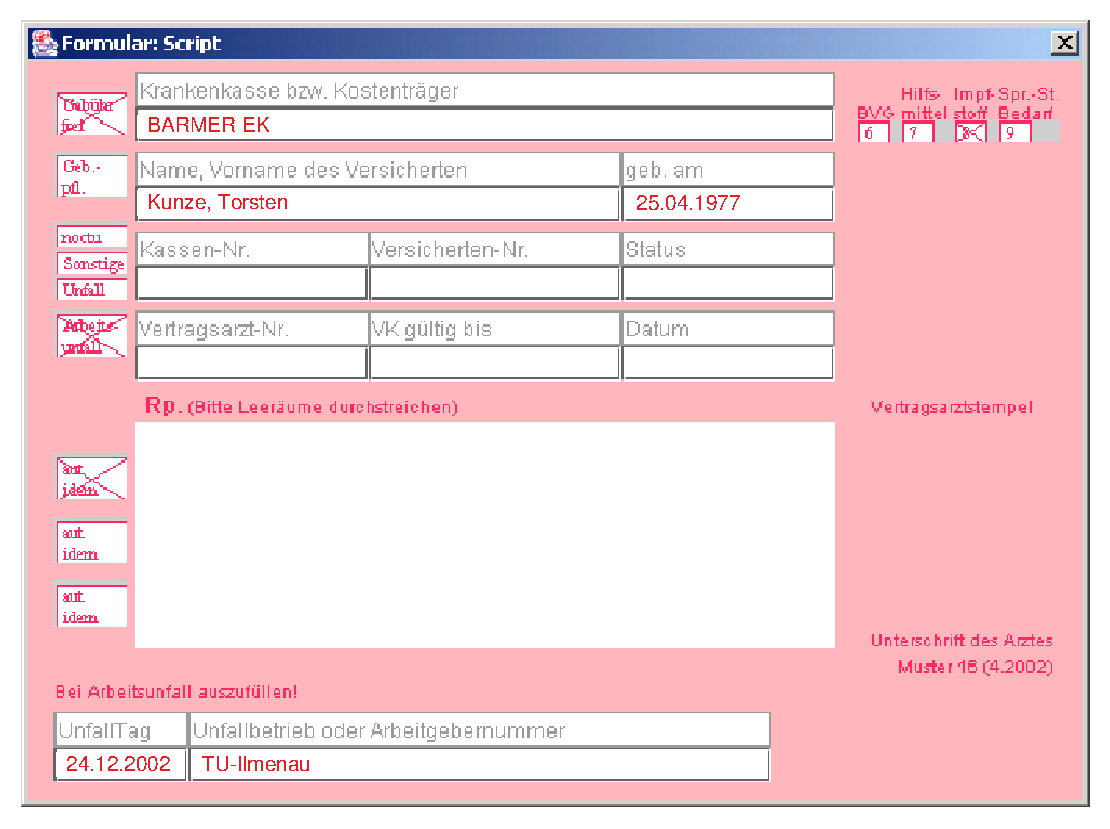
\includegraphics[scale=0.8]{Bilder/Formular_Rezept.eps}
  %     \caption{Das Rezept - Formular}
  %     \label{fig:Ein Formular - Rezept}
 %   \end{center}
%\end{figure}

\incljpg{0 0 403 296}{Bilder/Formular_Rezept.jpg}{Das Rezept - Formular}{Das Rezept -
Formular}{fig:Ein Formular - Rezept}

\section{Drucken der Formulare}
Um das Drucken nicht nur auf die Formulare zu beschr�nken, sondern f�r beliebige Anwendungsbereiche
zug�nglich zu halten, wurde die Funktionalit�t von den Formularelternklassen separiert und eine
spezialisierte Klasse erstellt, die diese Aufgabe bewerkstelligt.\\
Es bieten sich zwei M�glichkeiten des Druckens.\\
Zum einen kann eine Java-Swing-Komponente unmittelbar an diese Klasse �bergeben werden. Bei
Einhaltung des Design-Pattern Model View Controller handelt es sich hierbei um den aktuellen
Zustand des jeweiligen View-Objektes. Dieses wird bei Bedarf, sofern es den bedruckbaren Bereich
des Papierformates �berschreitet, herunterskaliert. Dabei offenbart sich der Nachteil des
Verfahrens, denn mit dem Skalieren werden Schrift und View-Komponenten meist stark verzerrt, da
Java keine optimierten Bildbearbeitungsoperationen zur Verf�gung stellt. Nach M�glichkeit sollten
deshalb nur Views gedruckt werden, die vollst�ndig auf das gew�hlte Papierformat passen.\\
Diese Variante erf�llt nicht die Anforderungen des \emph{ReForm}-Moduls, daher wurde noch eine
Weitere evaluiert. Sie setzt die Existenz einer eigens hierf�r zust�ndigen Methode im View voraus,
welche eine Maske zum Drucken von Text und anderen Swing-Komponenten erstellt. Damit wird nicht
mehr der vollst�ndige View ausgegeben, vielmehr kann man in vorgefertigte Standardformulare drucken
und diese Maske entsprechend des Papierformates gestalten. Der Nachteil ist ein erweiterter
Implementierungsaufwand f�r die Masken-Methode. Diese zweite Variante kommt bei \emph{ReForm} zum
Einsatz.
